\documentclass[conference,a4paper,10pt]{IEEETran}

\usepackage{amsmath,amssymb,amsfonts}
\usepackage{algorithmic}
\usepackage{graphicx}
\usepackage{textcomp}
\usepackage{xcolor}
\usepackage[utf8]{inputenc}
\usepackage{multirow}
\usepackage{setspace}
\usepackage{pdfpages}
\usepackage{float}
\usepackage{caption,newfloat}
\usepackage[utf8]{inputenc}
\usepackage{textgreek}
\usepackage[T1]{fontenc}
\usepackage[brazilian]{babel}
\usepackage[utf8]{inputenc}
\usepackage{ifthen}
\usepackage{tabularx}
\usepackage[pages=some]{background}
\RequirePackage[obeyspaces,hyphens]{url}
\RequirePackage[plainpages,pdfpagelabels]{hyperref}	% PDF com links, metadados
\RequirePackage{bookmark}				% cria um índice no PDF
\RequirePackage{microtype}	% melhorar a qualidade da tipografia no PDF
\usepackage{tabularx}
\usepackage{array}
\usepackage{caption}
\usepackage{float}
\usepackage{placeins}
\usepackage{pdfpages}



%% TODO
%% Se alguma hifenização não funcionar, adicionar aqui
\hyphenation{di-gi-ta-li-za-das}


%%%%%%%%%%%%%%%%%%%%%%%%%%%%%%%%%%%%%%%%%%%%%%%%%%%%%%%%%%%%%%%%%%%%%%%%
%     INÍCIO DO DOCUMENTO
%%%%%%%%%%%%%%%%%%%%%%%%%%%%%%%%%%%%%%%%%%%%%%%%%%%%%%%%%%%%%%%%%%%%%%%%
\begin{document}

%%%% NÃO MEXER NESTES ARQUIVOS
%%%% Definições/Estilos customizadas para o TADS, Mais capa
% \captionsetup{
%    tablename=TABELA,
%    listformat=empty,
%    justification=centering,
%    %labelsep=newline,
%    position=above,
%    skip=0.2\baselineskip,
%    width=\linewidth,
%    labelfont={small},
%    font={small} 
% }

\newcommand{\legenda}[1]{\caption{#1}}

\pagenumbering{arabic}

\def\BibTeX{{\rm B\kern-.05em{\sc i\kern-.025em b}\kern-.08em
    T\kern-.1667em\lower.7ex\hbox{E}\kern-.125emX}}

\newcommand{\tabelaname}{TABELA}
\newcommand{\figuraname}{FIGURA}
\newcommand{\quadroname}{QUADRO}
\newcounter{quadrocounter}
\setcounter{quadrocounter}{0}
% posicao, legenda, fonte
\newenvironment{quadro}[4][!t]
{
  \refstepcounter{quadrocounter}
  \label{#4}
  \def\fonteval{#3}
  \begin{table}[#1]
    \begin{center}
      % legenda
      \par\medskip\noindent
      QUADRO~\thequadrocounter~-~#2
      \par\medskip\noindent
}
{
      \par\noindent
      \fonte{\fonteval}
    \end{center}
  \end{table}
}
\newenvironment{quadro*}[4][!t]
{
  \refstepcounter{quadrocounter}
  \label{#4}
  \def\fonteval{#3}
  \begin{table*}[#1]
    \begin{center}
      % legenda
      \par\medskip\noindent
      QUADRO~\thequadrocounter~-~#2
      \par\medskip\noindent
}
{
      \par\noindent
      \fonte{\fonteval}
    \end{center}
  \end{table*}
}

\newcounter{tabelacounter}
\setcounter{tabelacounter}{0}
\newenvironment{tabela}[4][!t]
{
  \refstepcounter{tabelacounter}
  \label{#4}
  \def\fonteval{#3}
  \begin{table}[#1]
    \begin{center}
      % legenda
      \par\medskip\noindent
      TABELA~\thetabelacounter~-~#2
      \par\medskip\noindent
}
{
      \par\noindent
      \fonte{\fonteval}
    \end{center}
  \end{table}
}
\newenvironment{tabela*}[3][!t]
{
  \refstepcounter{tabelacounter}
  \def\fonteval{#3}
  \begin{table*}[#1]
    \begin{center}
      % legenda
      \par\medskip\noindent
      TABELA~\thetabelacounter~-~#2
      \par\medskip\noindent
}
{
      \par\noindent
      \fonte{\fonteval}
    \end{center}
  \end{table*}
}
\newcounter{figuracounter}
\setcounter{figuracounter}{0}
\newenvironment{figura}[4][!t]
{
  \def\fonteval{#3}
  \refstepcounter{figuracounter}
  \label{#4}
  \begin{figure}[#1]
    \begin{center}
      % legenda
      \par\medskip\noindent
      FIGURA~\thefiguracounter~-~#2
      \par\medskip\noindent
}
{
    \par\noindent
    \fonte{\fonteval}
    \end{center}
  \end{figure}
}
\newenvironment{figura*}[4][!t]
{
  \refstepcounter{figuracounter}
  \label{#4}
  \def\fonteval{#3}
  \begin{figure}[#1]
    \begin{center}
    % legenda
    \par\medskip\noindent
    FIGURA~\thefiguracounter~-~#2
    \par\medskip\noindent
}
{
    \par\noindent
    \fonte{\fonteval}
  \end{center}
  \end{figure}
}

\newcommand*{\captionsource}[2]{%
  \caption[{#1}]{%
  \centering
    #1%
    \hspace{\linewidth}%
    FONTE: #2%
  }%
}

\newcommand*{\fonte}[1]{%
  \centering
  \small
  \vspace{1em}
  \hspace{\linewidth}%
  FONTE: #1%
}

\def\abstractname{Abstract: }


%%%%%%%%%%%% CONFIGURAÇÃO DA CAPA E FOLHA DE ROSTO %%%%%%%%%%%%%%

\def\descr{Trabalho de conclusão de curso apresentado ao
curso de graduação em Análise e
Desenvolvimento de Sistemas, Setor de Educação
Profissional e Tecnológica, Universidade Federal
do Paraná, como requisito parcial à obtenção do
título de tecnólogo}



%%%% fundo na capa

\backgroundsetup{
scale=1,
color=black,
opacity=0.4,
angle=0,
contents={%
  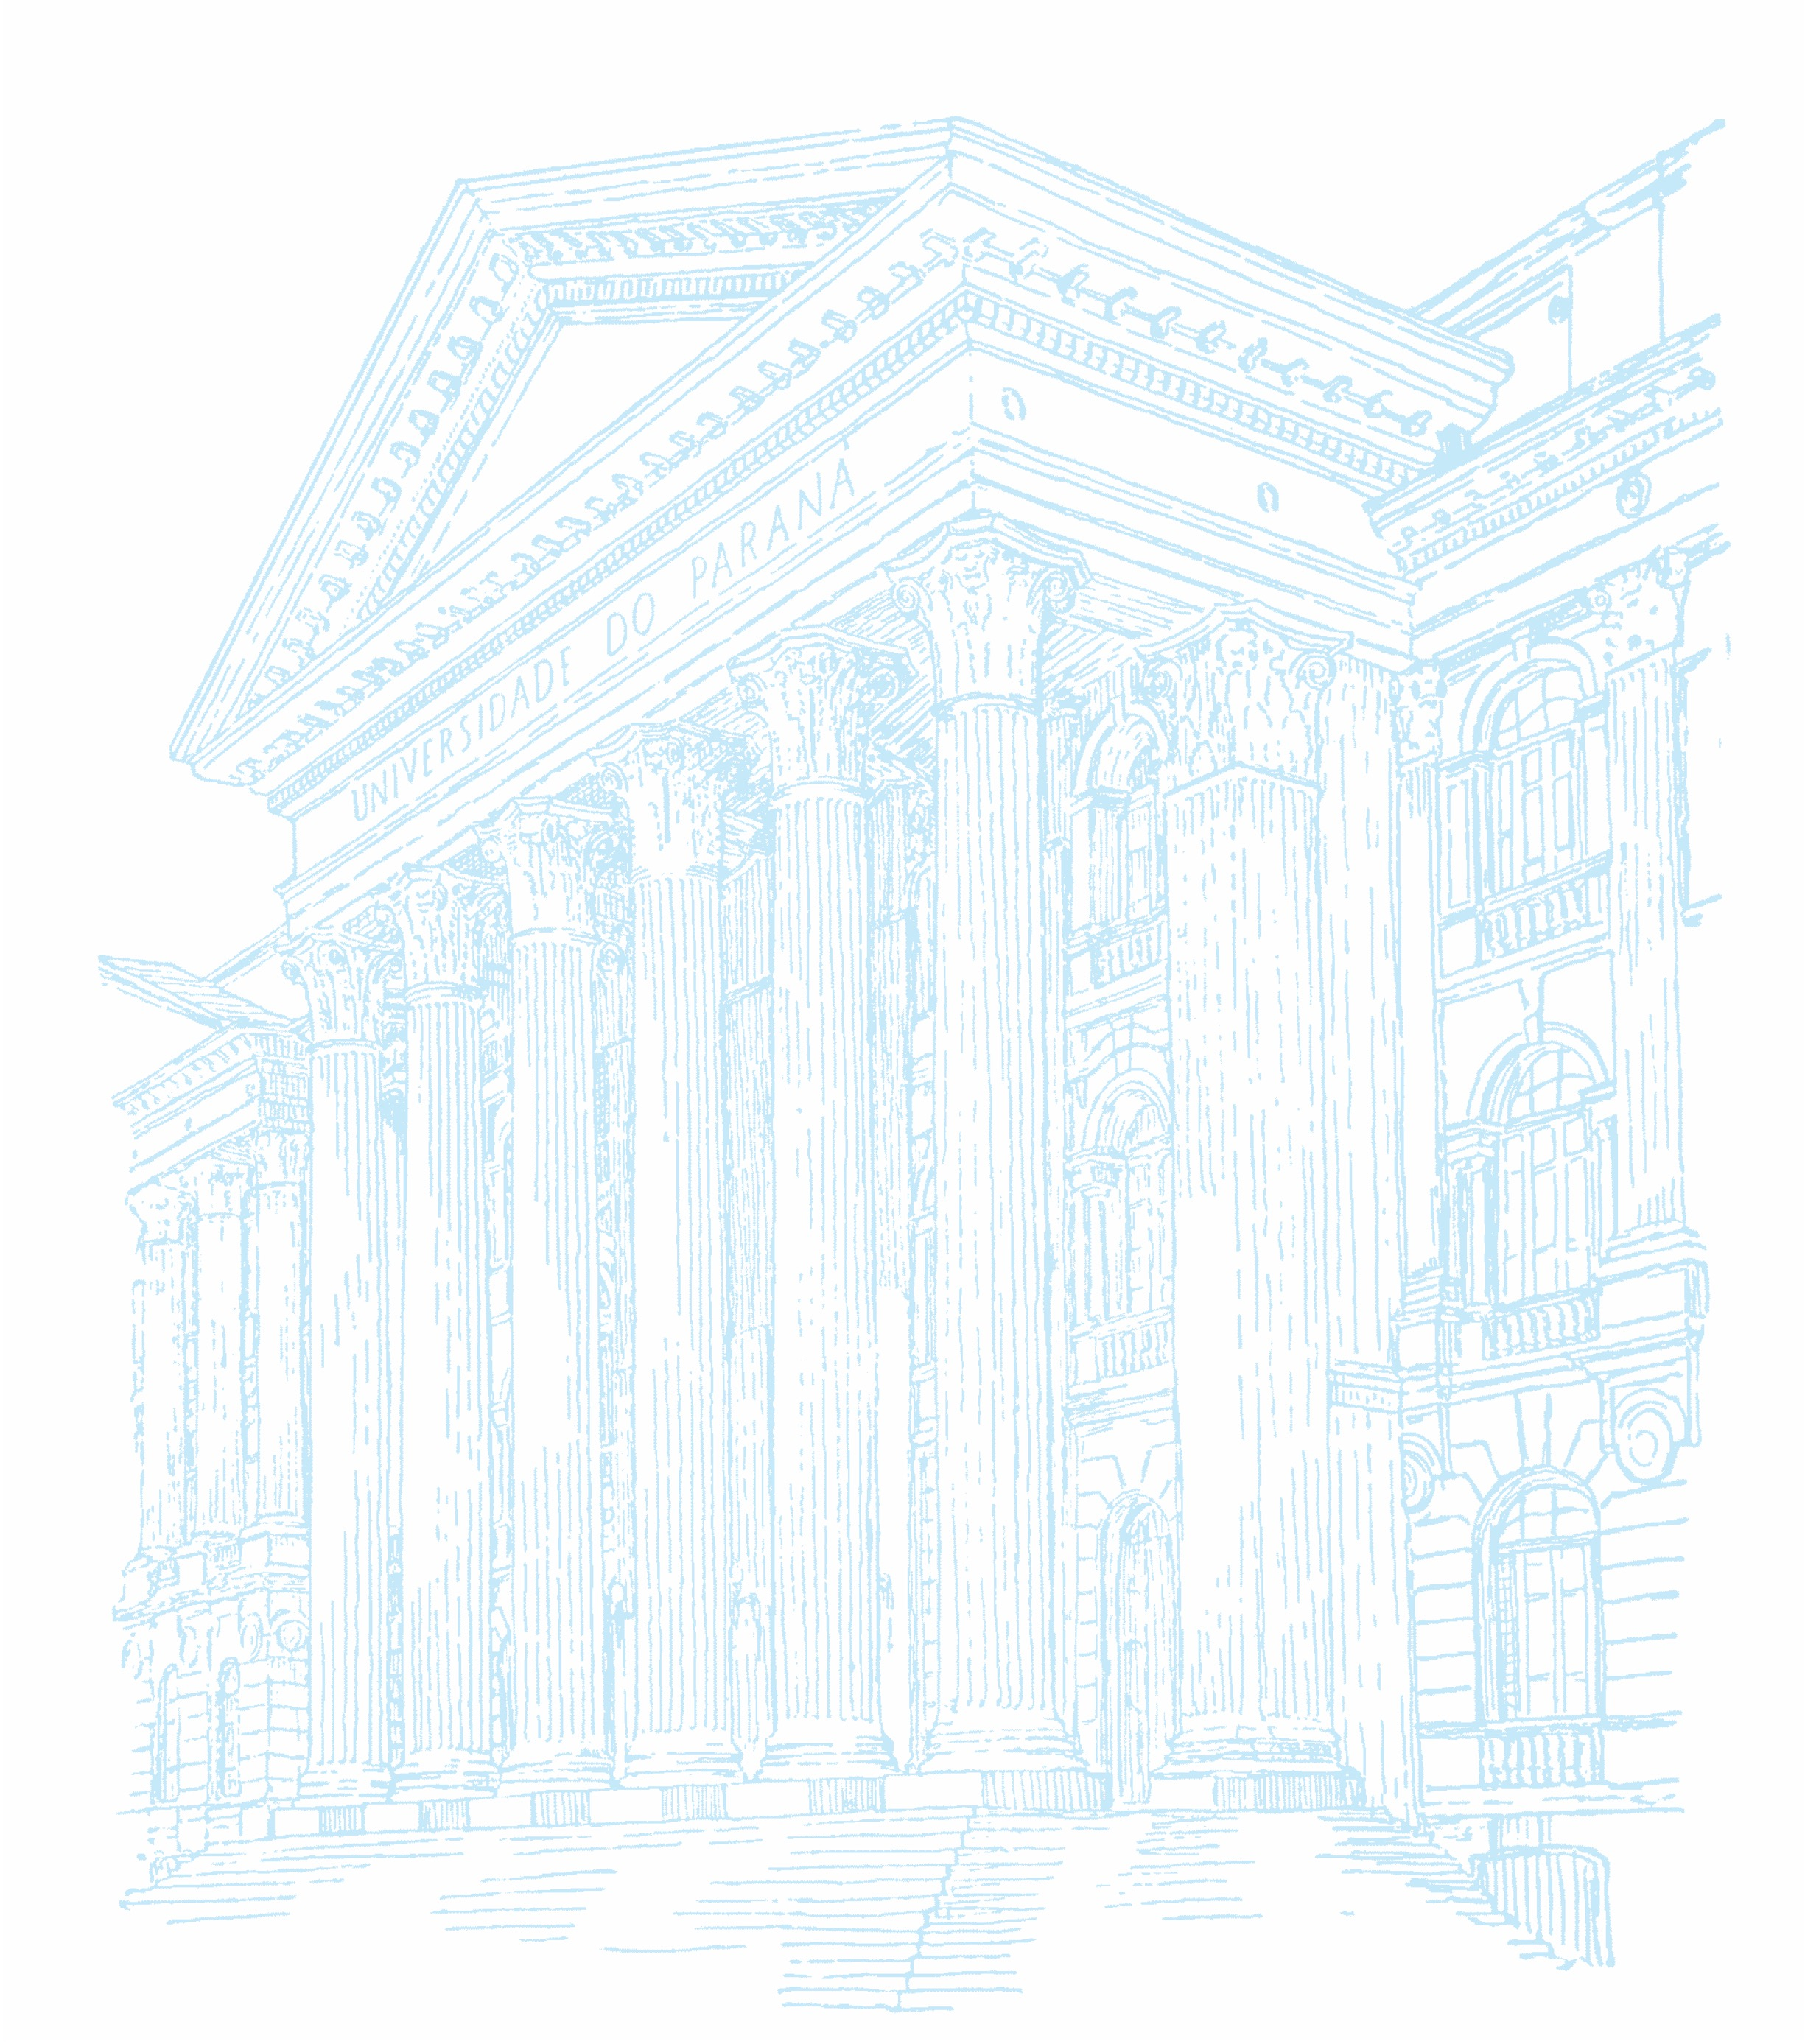
\includegraphics[width=\paperwidth,height=\paperheight]{bg_capa.jpg}
  }%
}
%%%%


%%%%%%% Definição da capa e folha de rosto


%\fancypagestyle{frontmatter}{
%  \fancyhf{}
%}

%\fancypagestyle{plain}{
%  \fancyhf{}
%  \if@mainmatter
%    \if@twoside
%      \fancyhead[LE,RO]{\thepage}
%    \else
%      \fancyhead[R]{\thepage}
%    \fi
%  \fi
%}



\hypersetup{
  % pdftitle, author, etc definidos mais abaixo
%  bookmarks   = true,
%  pageanchor  = false,
  hypertexnames = false,
%  bookmarkstype = page,
  pdfview     = Fit,
  pdfborder   = {0 0 0},
  colorlinks  = false,
  linkcolor   = blue,
  anchorcolor = blue,
  citecolor   = blue,
  filecolor   = blue,
%  pagecolor   = blue,
  urlcolor    = blue
}




%\def\@advisor{}			% orientador
%\def\@coadvisor{}		% co-orientador
%\def\@local{}			% local
%\def\@descr{}			% descrição do documento
%\def\@pcs{}			% palavras-chave
%\def\@kws{}			% keywords


%\newcommand{\autorcapa}[1]{\def\@author{#1}}
%\renewcommand{\title}[1]{\def\@title{#1}}

% descrição do documento na folha de rosto
%\newcommand{\descr}[1]{\def\@descr{#1}}

% orientadores
%\newcommand{\advisor}[1]{\def\@advisor{#1}}
%\newcommand{\coadvisor}[1]{\def\@coadvisor{#1}}


% local (cidade)
%\newcommand{\local}[1]{\def\@local{#1}}

\newcommand{\capa}[1]
{
  % páginas iniciais não são numeradas
  %\pagestyle{empty}
  %\thispagestyle{empty}

  % ajustar tags do PDF final
  \hypersetup{
    pdftitle    = {\titulo},
    pdfproducer = {UFPR - Universidade Federal do Paraná}
  }

  % primeira capa (só na versão aprovada)
  %\iffinalmode
%    \phantomsection
%    \thispagestyle{empty}

    \BgThispage
    
    \begin{center}
      \begin{doublespace}
        \textsc{\Large{UNIVERSIDADE FEDERAL DO PARANÁ}}
        \par
        \vspace{2cm}
        #1
        \vfill
        \DeclareRobustCommand\\{\linebreak}
        \textsc{\Large\titulo}
        \vfill
        \textsc{\Large\local\\\ano}
      \end{doublespace}
    \end{center}
    \cleardoublepage
    
    
  %\fi

  % folha de rosto
  \clearpage
%  \phantomsection
%  \addcontentsline{toc}{chapter}{Rosto}
%  \thispagestyle{empty}

  % autor
  \begin{center}
      \begin{doublespace}
        #1
      \end{doublespace}
  \end{center}

  \vfill\vfill

  % título
  \begin{doublespace}
    \begin{center}
      \DeclareRobustCommand\\{\linebreak }
      \textsc{\Large\titulo}
    \end{center}
  \end{doublespace}

  \vspace{1cm}

  % selo descritivo
  \hfill
  \begin{minipage}{9cm}

    % descrição
    \ifx\descr\@empty
    \else
      \descr.
    \fi

    % orientador
    \ifx\orientador\@empty
    \else
      \vspace{1em}
      Orientador: \orientadornome.
    \fi

    % coorientador
    \ifx\coorientador\undefined
    \else
      \vspace{1em}
      Co-orientador: \coorientador.
    \fi

  \end{minipage}

  \vfill

  % local e data
  \begin{center}
    \begin{doublespace}
      \textsc{\Large\local\\\ano}
    \end{doublespace}
  \end{center}

  % that's all, folks!
  \cleardoublepage
}


\newcommand{\termoaprovacao}
{
    \begin{center}
      \begin{doublespace}
        \vfill
        \Large{Substituir esta página pelo Termo de Aprovação que será fornecido após a defesa.}
        \vfill
      \end{doublespace}
    \end{center}
    \cleardoublepage
    
}

% \newcommand{\linebreakand}{%
%   \end{@IEEEauthorhalign}
%   \hfill\mbox{}\par
%   \mbox{}\hfill\begin{@IEEEauthorhalign}
% }

\newcommand*{\refmark}[1]{\raisebox{0pt}[0pt][0pt]{\textsuperscript{\footnotesize #1}}}
\newcommand{\autores}[1]{
  \author{
      \IEEEauthorblockN{
        #1
      }
      %\IEEEauthorblockN{#1\refmark{1}, #2\refmark{1}, #3\refmark{1}, #4\refmark{1}, #5\refmark{1}}
      \IEEEauthorblockA{\refmark{1}\textit{\setor} \\ \textit{\ufpr} }
  }
}

%%%%%%%



%%%%%%%%%%%%%%%%%%%%%%%%%%%%%%%%%%%%%%%%%%%%%%%%%%%%%%%%%%%%%%%%%%%%%%%%
%%%% Definições usadas para geração da capa, folha de rosto e títulos
%% TODO Alterar para seu trabalho
\def\autorescapa{
    \textsc{\Large GABRIEL HENRIQUE SPERANCETA}\\
    \textsc{\Large JOÃO PEDRO COSTA GUERIOS}\\
    \textsc{\Large LUCCA HAJ MUSSI CHELLA PARANHOS SILVA}\\
    \textsc{\Large WESLEY PARASTCHUK}\\
}

\def\autorestitulo{
  Gabriel Henrique Speranceta\refmark{1}, João Pedro Costa Guerios\refmark{1}, Lucca Haj Mussi Chella Paranhos Silva\refmark{1},\\
  Wesley Parastchuk\refmark{1}
}

\def\titulo{Sistema de Acompanhamento para Pessoas com Alzheimer}

\def\repositorio{https://bibliotecas.ufpr.br/}

\def\orientadornome{Prof. Dr. Alessandro Brawerman}
\def\orientadoremail{brawerman@ufpr.br}


\def\local{Curitiba, PR}
\def\ano{2025}
\def\setor{Setor de Educação Profissional e Tecnológica}
\def\ufpr{Universidade Federal do Paraná}
\def\cidade{Curitiba, Brasil}
%%%%%%%%%%%%%%%%%%%%%%%%%%%%%%%%%%%%%%%%%%%%%%%%%%%%%%%%%%%%%%%%%%%%%%%%


%% Cria a capa em 1 coluna
\onecolumn

%%%%%%%%%%%%%%%%%%%%%%%%%%%%%%%%%%%%%%%%%%%%
% TODO : Adicionar o nome dos alunos aqui
\capa{\autorescapa}

%% Inclusão do Termo de Aprovação
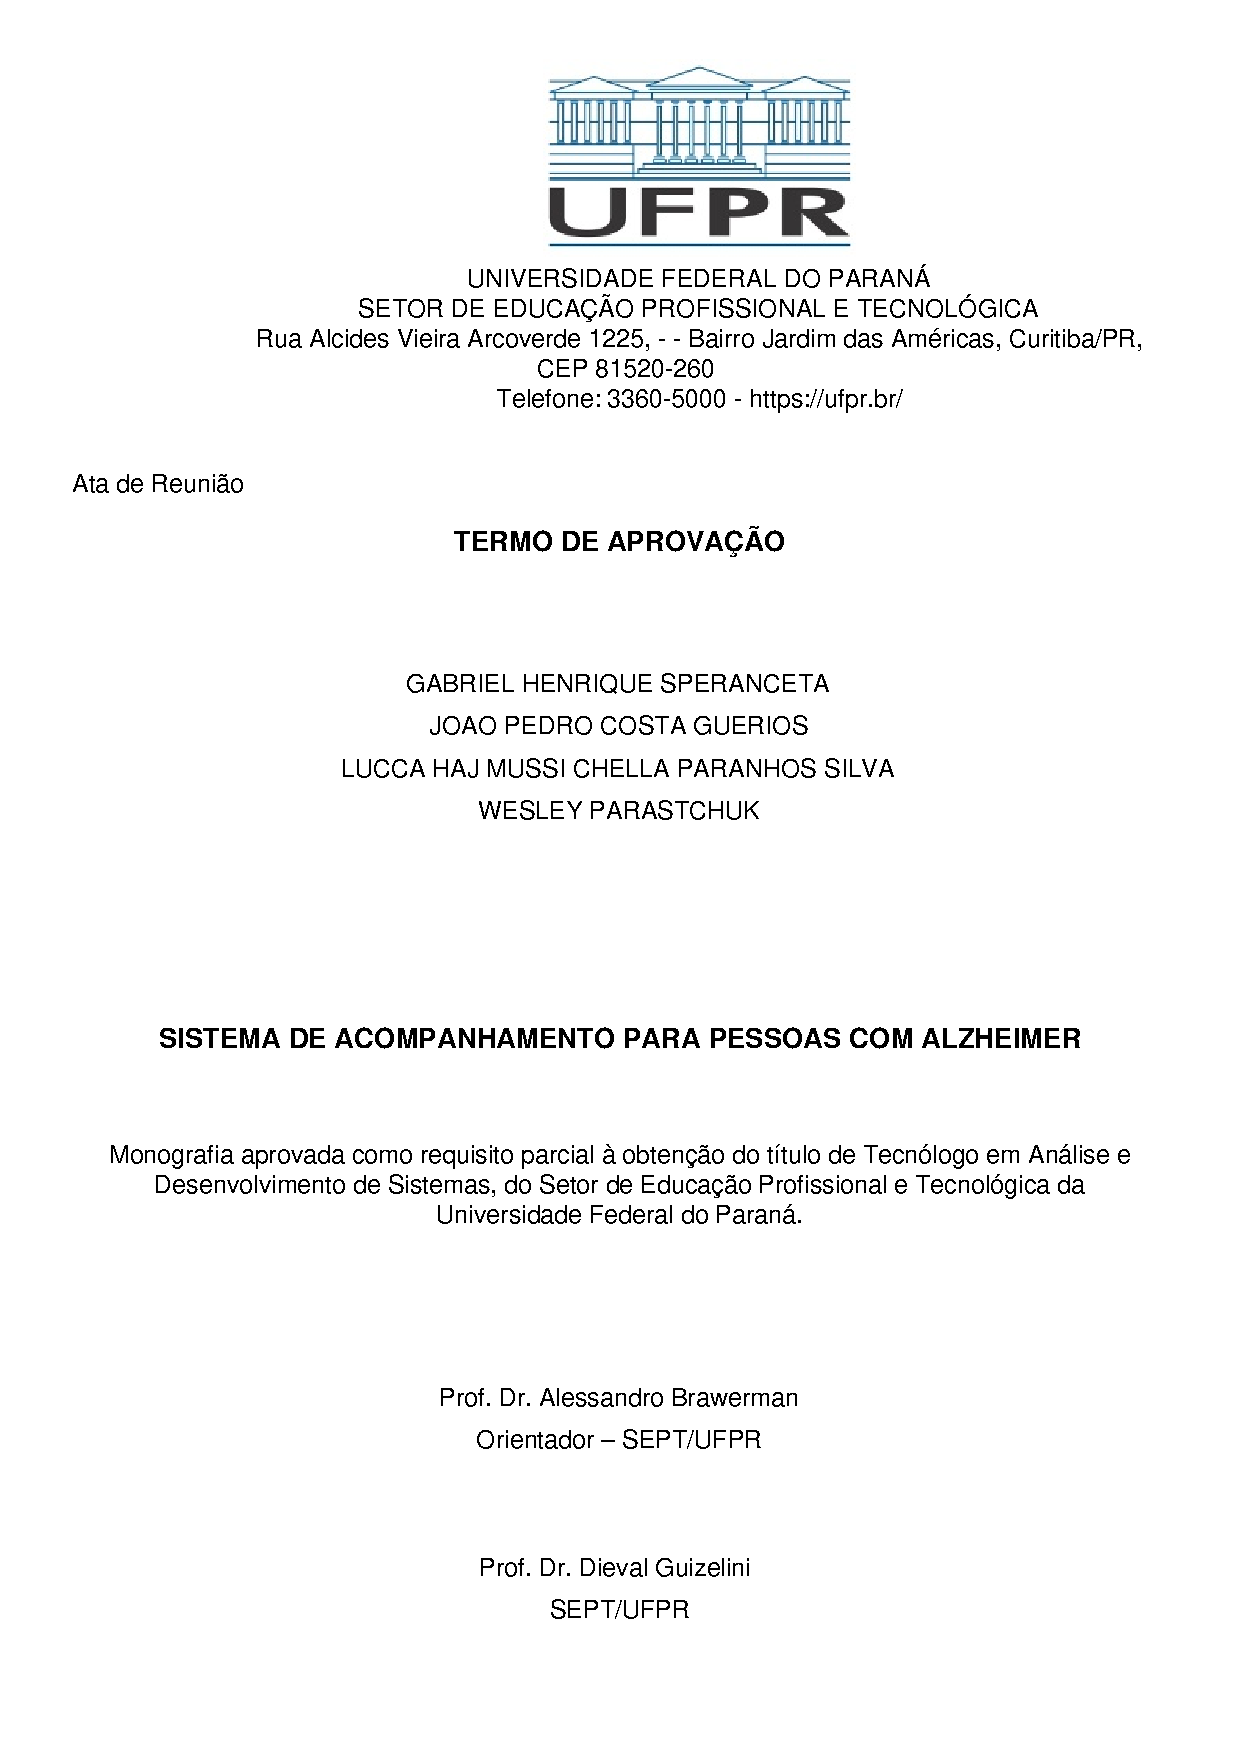
\includepdf[pages=-]{SEI_8458158_Ata_de_Reuniao.pdf}

%% Cria o título do artigo
\twocolumn
\title{\titulo}

%%%%%%%%%%%%%%%%%%%%%%%%%%%%%%%%%%%%%%%%%%%%
\autores{\autorestitulo}

\maketitle

\thispagestyle{plain}
\pagestyle{plain}

%%%%%%%%%%%%%%%%%%%%%%%%%%%%%%%%%%%%%%%%%%%%%%%%%%%%%%%%%%%%
% Resumo e palavras-chave
\begin{resumo}
A Doença de Alzheimer representa um desafio crescente para os sistemas de saúde globais e para as famílias, dada a sua progressão lenta e o impacto significativo na autonomia dos pacientes. A variabilidade na deterioração cognitiva exige um monitoramento contínuo e detalhado, que muitas vezes é difícil de ser alcançado com métodos tradicionais, aumentando o estresse dos cuidadores e comprometendo a segurança do paciente. Este trabalho teve como objetivo geral o desenvolvimento de um sistema de acompanhamento integrado para pessoas com Alzheimer, visando melhorar o monitoramento, a comunicação entre médicos, pacientes e cuidadores, e a gestão do tratamento por meio de uma solução tecnológica. O projeto consiste em uma plataforma web e um aplicativo móvel que centralizam o fluxo de informações, permitindo o registro de exames, a comunicação direta e a organização clínica via dashboard e adição de conslusões conforme o andamento do tratamento. Especificamente, a plataforma web permite ao corpo médico o gerenciamento de pacientes e a visualização do histórico completo, enquanto o aplicativo móvel facilita para pacientes e cuidadores o envio de resultados e o contato imediato via chat. A metodologia de desenvolvimento adotada foi o Scrum, organizada em Sprints que garantiram entregas incrementais do produto. A arquitetura do sistema foi implementada na nuvem da Microsoft Azure, utilizando tecnologias como React e React Native para as interfaces, e Java com Spring Boot para a construção da API, assegurando uma solução robusta, escalável e segura. Como resultado, o sistema oferece uma ferramenta eficaz para otimizar o cuidado, promover a intervenção rápida e melhorar a qualidade de vida dos envolvidos no tratamento da Doença de Alzheimer.
\end{resumo}

\begin{palavraschave}
Alzheimer; Sistema de Acompanhamento; Nuvem.
\end{palavraschave}

%%%%%%%%%%%%%%%%%%%%%%%%%%%%%%%%%%%%%%%%%%%%%%%%%%%%%%%%%%%%
% Abstract e keywords
\begin{abstract}
Alzheimer's disease represents a growing challenge for global health systems and families, given its slow progression and significant impact on patient autonomy. The variability in cognitive deterioration requires continuous and detailed monitoring, which is often difficult to achieve with traditional methods, increasing caregiver stress and compromising patient safety. The general objective of this work was to develop an integrated follow-up system for people with Alzheimer's, aiming to improve monitoring, communication between doctors, patients, and caregivers, and treatment management through a technological solution. The project consists of a web platform and a mobile application that centralize the flow of information, allowing for the registration of exams, direct communication, clinical organization via a dashboard, and the addition of conclusions as the treatment progresses. Specifically, the web platform allows the medical team to manage patients and view their complete history, while the mobile application facilitates the submission of results and immediate contact via chat for patients and caregivers. The development methodology adopted was Scrum, organized into Sprints that ensured incremental product deliveries. The system architecture was implemented on the Microsoft Azure cloud, using technologies such as React and React Native for the interfaces, and Java with Spring Boot for the API construction, ensuring a robust, scalable, and secure solution. As a result, the system offers an effective tool to optimize care, promote rapid intervention, and improve the quality of life for those involved in the treatment of Alzheimer's disease.
\end{abstract}

\begin{keywords}
Alzheimer; Tracking system; Cloud.
\end{keywords}


%%%%%%%%%%%%%%%%%%%%%%%%%%%%%%%%%%%%%%%%%%%%%%%%%%%%%%%%%%%%
% Início do documento propriamente dito

\section{INTRODUÇÃO}

O estudo da Doença de Alzheimer se mostra cada vez mais relevante diante do crescente número de casos e do impacto multifatorial que a doença acarreta. Trata-se de uma condição que compromete não apenas a autonomia e qualidade de vida dos pacientes, mas também representa um enorme desafio para familiares, cuidadores, profissionais da saúde e para os sistemas públicos e privados de saúde. Além disso, compreender os mecanismos fisiopatológicos da doença, bem como desenvolver estratégias para diagnóstico precoce, tratamento e monitoramento, é fundamental para mitigar os efeitos sociais, emocionais e econômicos associados ao Alzheimer \cite{Scheltens2021Alzheimer}. O avanço tecnológico, aliado ao uso de sistemas inteligentes de apoio à decisão, representa uma oportunidade promissora para melhorar o cuidado com esses pacientes.

%\subsection{Problema}
A progressão da Doença de Alzheimer é lenta e a deterioração cognitiva varia
consideravelmente entre os pacientes \cite{Scheltens2021Alzheimer}. Essa variabilidade exige um monitoramento
contínuo para identificar pequenas mudanças que sinalizem o avanço da doença,
permitindo ajustes oportunos nas intervenções médicas e comportamentais. A falta de
um acompanhamento detalhado que capture variações nos comportamentos diários
impede a antecipação de eventos perigosos, como agitação ou desorientação. Isso
não apenas compromete a segurança e o bem-estar do paciente, mas também
aumenta o estresse e a sobrecarga emocional dos cuidadores, que necessitam de
ferramentas eficazes para uma intervenção rápida \cite{carvalho_Clinical, lv_iCare}.

%\subsection{Objetivo geral}
Este trabalho apresenta o desenvolvimento de um sistema de acompanhamento para pessoas com Alzheimer, visando melhorar o monitoramento contínuo, a comunicação entre médicos, pacientes e cuidadores, e a gestão do tratamento por meio de uma solução tecnológica integrada. O sistema é composto por uma plataforma web voltada para o corpo médico, que permite o gerenciamento de pacientes, a solicitação de exames, o registro de conclusões e a visualização de um dashboard com indicadores e histórico clínico completo. Além disso, inclui um aplicativo móvel para pacientes e seus cuidadores, facilitando o envio de exames, o anexo de histórico médico pregresso e o acompanhamento das requisições. A solução conta ainda com funcionalidades de chat, para viabilizar a comunicação direta entre as partes, e um sistema de notificações automatizado para informar sobre novas solicitações, conclusões e atualizações no status do tratamento.

%\subsection{Justificativa}
A relevância deste projeto é sustentada pelo cenário epidemiológico global e nacional da Doença de Alzheimer. De acordo com a Organização Mundial da Saúde (OMS), mais de 55 milhões de pessoas vivem com algum tipo de demência mundialmente, com o Alzheimer sendo responsável por 60\% a 70\% desses casos. As projeções indicam que, sem avanços significativos na prevenção e tratamento, esse número pode ultrapassar 150 milhões até 2050 devido ao envelhecimento populacional \cite{Scheltens2021Alzheimer}.

No Brasil, a Associação Brasileira de Alzheimer (ABRAz) informa que aproximadamente 1,2 milhão de pessoas convivem com a doença, com cerca de 100 mil novos casos surgindo anualmente \cite{BVSMS2023Alzheimer}. Este contexto evidencia a necessidade urgente de políticas públicas, investimento em pesquisa \cite{drew_Alzheimers, Makin2025Dementia, FDA2023Alzheimers} e, crucialmente, a adoção de tecnologias inovadoras que auxiliem no diagnóstico e no cuidado de pessoas com Alzheimer. A utilização de uma solução digital, como a proposta neste trabalho, pode otimizar o monitoramento, facilitar a comunicação e oferecer um suporte mais eficaz tanto para os pacientes quanto para seus cuidadores, alinhando-se à crescente transformação digital no setor da saúde \cite{carvalho_Clinical, lv_iCare, Shah2023ReactNative}.

Este documento está organizado em cinco seções que detalham o desenvolvimento do projeto. A Seção 2 apresenta a fundamentação teórica, abordando os aspectos médicos e científicos da Doença de Alzheimer, as estratégias de progressão e monitoramento, bem como os fundamentos tecnológicos para o desenvolvimento de soluções em saúde digital. A Seção 3 descreve a metodologia de desenvolvimento adotada, baseada em práticas ágeis e modelagem de software, além de detalhar as ferramentas e tecnologias utilizadas na construção da arquitetura do sistema. Na Seção 4, são apresentados os resultados obtidos, com a descrição da arquitetura implementada na nuvem Microsoft Azure e a demonstração das funcionalidades e interfaces dos sistemas Web e Mobile. Por fim, a Seção 5 traz as considerações finais, discutindo o atendimento aos objetivos propostos, as limitações do escopo atual e as perspectivas para trabalhos futuros.



%=============================================================================%
%============================== Secao 2 ======================================%
%=============================================================================%

\section{REVISÃO DE LITERATURA}\label{sec:revlit}
A Doença de Alzheimer (DA) representa um desafio global crescente, impactando a autonomia dos pacientes e gerando sobrecarga aos sistemas de saúde e familiares. Com o envelhecimento populacional, a OMS estima que os casos de demência (sendo 60\% a 70\% Alzheimer) saltem de 55 milhões para 150 milhões até 2050 \cite{Scheltens2021Alzheimer}. No Brasil, estima-se 1,2 milhão de casos atuais. A tecnologia e o uso de sistemas inteligentes surgem como oportunidades vitais para diagnóstico, tratamento e mitigação dos impactos socioeconômicos \cite{carvalho_Clinical}.

\subsection{Aspectos médicos e científicos}
A doença divide-se clinicamente em três fases principais \cite{Scheltens2021Alzheimer}. O estágio inicial é o \textbf{Pré-clínico}, marcado pela presença de alterações biológicas sem sintomas evidentes. Segue-se o \textbf{Comprometimento Cognitivo Leve (MCI)}, caracterizado por dificuldades cognitivas leves, mas com autonomia preservada nas atividades diárias. Por fim, a fase de \textbf{Demência} acarreta o comprometimento significativo da independência e qualidade de vida do paciente.

Para o reconhecimento dessas fases, o diagnóstico precoce depende de biomarcadores (do LCR e plasmáticos) que detectam níveis anormais de beta-amiloide (A\textbeta1-42) e Tau (t-tau, p-tau). Essas ferramentas permitem identificar a doença antes dos sintomas clínicos, sendo cruciais para a eficácia de tratamentos modificadores da doença e ensaios clínicos \cite{FDA2023Alzheimers, plasma_biomarkers, Scheltens2021Alzheimer}. Identificar a DA no início permite intervenções que desaceleram sintomas e preservam a autonomia \cite{FDA2023Alzheimers, Scheltens2021Alzheimer}. Além de diferenciar a demência de outras condições tratáveis, o diagnóstico precoce possibilita o planejamento familiar (financeiro e jurídico) e a redução da sobrecarga física e emocional dos cuidadores \cite{BVSMS2023Alzheimer, drew_Alzheimers}.

Quanto ao curso clínico, a evolução da DA é lenta e variável entre pacientes \cite{QiuPredictiveModeling, Sukkar2012Disease}. O monitoramento contínuo torna-se essencial para ajustar tratamentos e detectar mudanças sutis de comportamento. Acompanhar variações diárias ajuda a prever e evitar eventos perigosos, como episódios de agitação ou desorientação, permitindo intervenções rápidas \cite{lv_iCare, ChiarandiniWandering}.

No âmbito das intervenções, as abordagens terapêuticas dividem-se em inovações recentes e tratamentos tradicionais. Os **Anticorpos Monoclonais**, como Lecanemabe e Donanemabe, focam na redução de placas amiloides, desacelerando o declínio cognitivo em cerca de 30\% \cite{FDA2023Alzheimers, Makin2025Dementia}. Já os **Tratamentos Tradicionais** envolvem o uso de inibidores de colinesterase (ex: Donepezila) e Memantina para controle de sintomas e melhora na comunicação neuronal \cite{Scheltens2021Alzheimer}. Adicionalmente, o controle de fatores de risco modificáveis (como hipertensão e sedentarismo) pode prevenir uma parcela significativa dos casos.

\subsection{Contextos históricos e predições do Alzheimer}

O uso de históricos contextuais constitui um elemento fundamental no apoio ao acompanhamento e à predição da progressão da Doença de Alzheimer. Esses históricos são formados a partir da coleta contínua de dados fisiológicos, comportamentais e ambientais ao longo do tempo, permitindo a construção de perfis individuais dos pacientes e a identificação de padrões relevantes de comportamento e saúde \cite{lv_iCare}. Informações como variações no padrão de sono, níveis de atividade física, alterações de humor, localização e interação com o ambiente fornecem subsídios valiosos para análises preditivas mais precisas.

Nesse contexto, técnicas de Inteligência Artificial têm sido amplamente empregadas para modelar a natureza temporal e incerta desses dados. Redes Bayesianas, por exemplo, possibilitam a representação de relações probabilísticas entre diferentes variáveis clínicas e contextuais, auxiliando na inferência de estados de risco e na tomada de decisão clínica \cite{QiuPredictiveModeling}. De forma complementar, Modelos Ocultos de Markov (Hidden Markov Models – HMMs) são especialmente adequados para a análise de sequências temporais, permitindo inferir estados cognitivos não observáveis diretamente a partir de sinais observados \cite{Sukkar2012Disease}.

A aplicação dessas técnicas viabiliza a predição de eventos críticos, como episódios de agitação, desorientação ou deambulação indevida (\textit{wandering}), possibilitando intervenções preventivas e a personalização do cuidado \cite{ChiarandiniWandering}. Dessa forma, o uso de modelos preditivos baseados em históricos contextuais contribui significativamente para o aumento da segurança do paciente, para a redução de riscos associados à progressão da doença e para o aprimoramento da qualidade de vida tanto dos pacientes quanto de seus cuidadores.


\subsection{Cenário tecnológico de aplicativos para saúde}
O mercado global de \textit{mHealth} encontra-se em vigorosa expansão, tendo sido avaliado em USD 103,71 bilhões em 2025, com projeção de alcançar USD 329,75 bilhões até 2030 \cite{mordor_mhealth_2025}. Esse crescimento é impulsionado pela popularização de \textit{smartphones}, integração de Inteligência Artificial e dispositivos vestíveis (\textit{wearables}), que viabilizam o monitoramento remoto de pacientes \cite{lv_iCare, carvalho_Clinical}. Nesse contexto, os aplicativos assumem um papel central na transformação digital, focando na gestão de doenças crônicas (como diabetes e hipertensão), telemedicina e suporte à adesão medicamentosa. Além de beneficiarem os pacientes, essas soluções tornaram-se ferramentas vitais para cuidadores e familiares, facilitando a comunicação com equipes médicas e o acompanhamento de dependentes, mitigando erros na tomada de decisão clínica \cite{brainInventor_ReactNative, ChiarandiniWandering}.
Especificamente no contexto da Doença de Alzheimer, a tecnologia evoluiu para integrar dados clínicos, comportamentais e ambientais, proporcionando uma visão holística do paciente. As soluções modernas buscam ultrapassar o simples registro de dados, utilizando algoritmos de Inteligência Artificial, como Redes Bayesianas e Modelos Ocultos de Markov (HMMs), para analisar históricos contextuais e identificar padrões individuais \cite{QiuPredictiveModeling, Sukkar2012Disease}. Tais tecnologias permitem prever riscos iminentes, como episódios de agitação, tentativas de fuga ou quedas, possibilitando intervenções proativas e personalizadas antes que crises ocorram \cite{ChiarandiniWandering}. Para viabilizar essas soluções, é fundamental uma arquitetura robusta baseada em serviços (\textit{web services} via APIs REST), que garante a interoperabilidade entre dispositivos móveis e servidores, assegurando a integridade e privacidade dos dados sensíveis por meio de protocolos de segurança e autenticação \cite{carvalho_Clinical}.

%=============================================================================%
%============================== Secao 3 ======================================%
%=============================================================================%

\section{MÉTODO E TECNOLOGIAS}
Esta seção apresenta as metodologias e ferramentas que foram utilizadas para o desenvolvimento do projeto proposto. 
Para garantir organização e eficiência, o desenvolvimento do software baseou-se em metodologias ágeis, com ênfase no framework Scrum \cite{Schwaber2020ScrumGuide}. Essa abordagem permitiu entregas contínuas e flexibilidade para lidar com mudanças de requisitos, assegurando a qualidade técnica preconizada pela Engenharia de Software \cite{Pressman2016Software, Sommerville2011Software}.

O projeto consistiu em uma fase de arquitetura, regida por 7 sprints, seguida pelo desenvolvimento incremental ao longo de 11 Sprints. O cronograma de desenvolvimento foi estruturado de forma evolutiva e progressiva a partir da configuração de infraestrutura e funcionalidades básicas até módulos complexos, como o ciclo de exames e análise médica. 
Para o monitoramento do fluxo de trabalho, utilizou-se o método Kanban, permitindo a visualização de tarefas e limitação do trabalho em progresso (WIP) \cite{anderson_kanban_2012}. Paralelamente, a modelagem do sistema seguiu o padrão UML (Unified Modeling Language) \cite{larman_UML, booch_UML}. Foram elaborados diagramas de Casos de Uso, Classes, Sequência e Entidade-Relacionamento (DER) para estruturar a lógica da aplicação e do banco de dados PostgreSQL \cite{PostgreSQL2024Docs}. A confecção desses artefatos foi realizada através de ferramentas online colaborativas, como Draw.io e Dbdiagram.io \cite{drawio_website, dbdiagram_website}.
A construção do sistema exigiu a integração de um conjunto de ferramentas e tecnologias modernas, selecionadas de forma estratégica para garantir robustez, escalabilidade, segurança e uma boa experiência de uso. Cada tecnologia adotada desempenha um papel específico dentro da arquitetura proposta, abrangendo desde o desenvolvimento das interfaces Web e \textit{mobile}, passando pela implementação da API, até a gestão da infraestrutura em nuvem e o armazenamento de dados. As principais ferramentas utilizadas no projeto, bem como suas características e funções nas diferentes camadas do sistema, são apresentadas de forma sintetizada na Tabela~\ref{tab:tecnologias}, evidenciando o papel de cada tecnologia no desenvolvimento e na sustentação da solução.

\begin{table}[H]
    \centering
    \caption{Tecnologias utilizadas no projeto.}
    \label{tab:tecnologias}
    
    \footnotesize 
    
    \begin{tabularx}{\columnwidth}{|p{0.3\columnwidth}|X|}
        \hline
        \textbf{Tecnologia} & \textbf{Descrição Resumida} \\ \hline
        React (Web) & Interface Web dinâmica baseada em componentes e DOM virtual. \\ \hline
        React Native (Mobile) & Desenvolvimento de apps nativos iOS/Android com código compartilhado. \\ \hline
        TypeScript & Superset do JavaScript com tipagem estática para maior segurança. \\ \hline
        Java & Linguagem orientada a objetos robusta e multiplataforma para a API. \\ \hline
        Spring Boot & Framework para criação simplificada de aplicações Java prontas para produção. \\ \hline
        PostgreSQL & Banco de dados relacional seguro com suporte a transações complexas. \\ \hline
        Azure & Ecossistema de nuvem com serviços gerenciados e segurança integrada. \\ \hline
        Azure Spring Apps & PaaS gerenciada e otimizada para implantação de serviços Spring Boot. \\ \hline
        Azure Database for PostgreSQL & Instância gerenciada com alta disponibilidade, backups e segurança. \\ \hline
        Azure App Service & Plataforma de hospedagem Web escalável com suporte a CI/CD. \\ \hline
        Firebase & Armazenamento em nuvem para arquivos não estruturados (exames/imagens). \\ \hline
    \end{tabularx}
    
    \vspace{2mm}
    {\footnotesize Fonte: Os autores (2025)}
\end{table}

%=============================================================================%
%============================== Secao 4 ======================================%
%=============================================================================%

\section{RESULTADOS}

Neste capítulo são apresentadas a arquitetura da aplicação, bem como os sistemas finais (Web e Mobile) e suas principais funcionalidades.

\subsection{Arquitetura do Sistema}

A arquitetura geral do sistema, conforme ilustrado na Figura~\ref{fig:arqSistema}, foi concebida como uma solução nativa em nuvem, estruturada em um modelo de três camadas: cliente, servidor e dados.A camada de cliente é composta por dois \textit{frontends} distintos: uma aplicação Web, desenvolvida em React e hospedada no Azure App Service, destinada aos profissionais de saúde; e uma aplicação \textit{mobile}, desenvolvida em React Native, voltada para pacientes e cuidadores.A camada de servidor concentra o núcleo da arquitetura, sendo composta por uma API desenvolvida em Java com Spring Boot e implantada no Azure Spring Apps. Essa API é responsável por centralizar a lógica de negócio do sistema, além de atuar como ponto de integração e gateway para os demais serviços da plataforma.
Por fim, a camada de dados, também representada na Figura~\ref{fig:arqSistema}, adota uma estratégia híbrida de armazenamento. Informações estruturadas, como dados de pacientes, exames e registros clínicos, são persistidas no Azure Database for PostgreSQL, enquanto dados não estruturados, como documentos em PDF e imagens, são armazenados no Firebase, garantindo maior flexibilidade e escalabilidade.

\begin{figure}[H]
    \centering
    \caption{Arquitetura geral do sistema.}
    \makebox[\columnwidth][c]{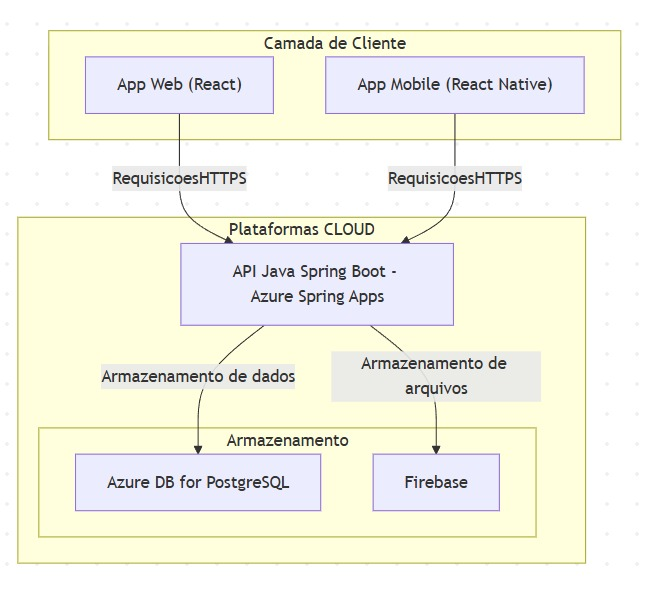
\includegraphics[height=8cm, keepaspectratio]{images/arq_geral.jpeg}}
    \label{fig:arqSistema}
    \vspace{2mm}
    {\footnotesize Fonte: Os autores (2025)}
\end{figure}

A aplicação Web, cuja arquitetura é apresentada na Figura~\ref{fig:arqWeb}, é implementada como uma \textit{Single-Page Application} (SPA) com o objetivo de fornecer aos médicos uma interface eficiente, responsiva e de fácil utilização. Desenvolvida em React com TypeScript e hospedada no Azure App Service, a aplicação adota uma arquitetura cliente–servidor baseada exclusivamente na comunicação via HTTPS.

Todas as interações com o backend ocorrem por meio de requisições no padrão RESTful, permitindo a execução das principais operações do sistema, tais como a consulta de dados clínicos dos pacientes, a visualização de exames e o acesso a documentos médicos. Essa abordagem favorece a separação de responsabilidades, a escalabilidade da aplicação e a manutenção do código, conforme evidenciado pelos componentes e fluxos descritos na Figura~\ref{fig:arqWeb}.

\begin{figure}[H]
    \centering
    \caption{Arquitetura do sistema Web.}
    \makebox[\columnwidth][c]{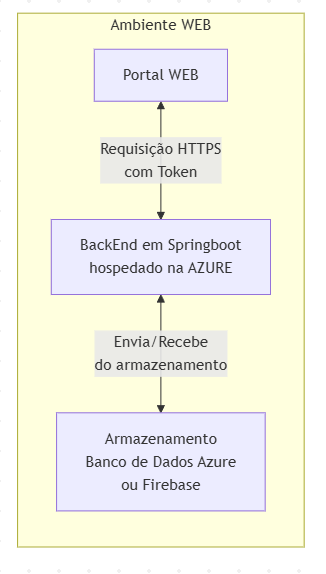
\includegraphics[height=8cm]{images/diagramas/arq_web_tcc_vertical.png}}
    \label{fig:arqWeb}
    \vspace{2mm}
    {\footnotesize Fonte: Os autores (2025)}
\end{figure}


O aplicativo \textit{mobile}, cuja arquitetura é apresentada na Figura~\ref{fig:arqMobile}, foi projetado com foco em simplicidade, acessibilidade e usabilidade, considerando as limitações cognitivas dos pacientes e a necessidade de praticidade para cuidadores. Desenvolvido em React Native com TypeScript, o aplicativo adota uma abordagem multiplataforma que permite o compartilhamento de código entre os sistemas Android e iOS.A comunicação com a camada de servidor ocorre por meio de requisições HTTP padrão no formato RESTful, garantindo a troca segura e eficiente de informações com o backend do sistema. Por meio dessa integração, o aplicativo possibilita o acesso a funcionalidades como o envio e a consulta de dados clínicos, notificações e acompanhamento de exames.Além disso, conforme ilustrado na Figura~\ref{fig:arqMobile}, a aplicação faz uso de recursos nativos dos dispositivos móveis, como a câmera e o sistema de arquivos, permitindo a captura e o envio de imagens e documentos relacionados aos exames médicos. Esses arquivos são armazenados de forma segura no Firebase Storage por meio da API do backend, assegurando escalabilidade, controle de acesso e integridade dos dados.


\begin{figure}[H]
    \centering
    \caption{Arquitetura do sistema Mobile.}
    % O makebox força a centralização dentro da largura da coluna
    \makebox[\columnwidth][c]{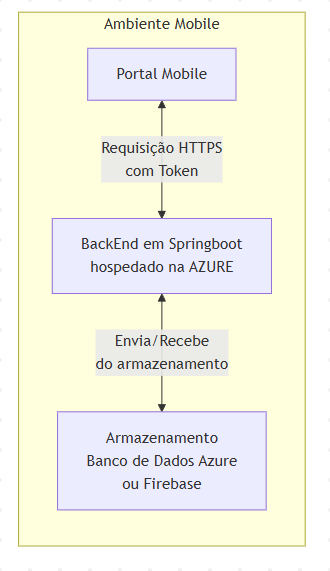
\includegraphics[height=7cm]{images/diagramas/arq_mobile_tcc_vertical.png}}
    \label{fig:arqMobile}
    \vspace{2mm}
    {\footnotesize Fonte: Os autores (2025)}
\end{figure}

\subsection{Apresentação do Sistema}
A interface do sistema foi projetada com foco em usabilidade e experiência do usuário (UX), seguindo diretrizes de acessibilidade para garantir operação intuitiva por pacientes idosos e seus cuidadores. A arquitetura contempla dois ambientes integrados e complementares: a plataforma Web, destinada ao corpo médico, e o aplicativo móvel, voltado a pacientes e familiares, permitindo fluxo contínuo de informação entre equipes clínicas e cuidadores.

\subsubsection{Plataforma Web (Visão do Médico)}
A plataforma Web é acessível apenas a profissionais autenticados, funcionando como o centro de controle clínico. A tela inicial oferece gerenciamento eficiente de pacientes com listagem organizada, filtros e busca por nome ou CPF, além de cadastro e edição de perfis. A navegação privilegia ações rápidas para triagem de pendências e priorização de casos. Adicionalmente, a plataforma disponibiliza um módulo de visualização de indicadores, responsável por apresentar métricas consolidadas relacionadas aos pacientes, exames, solicitações e evolução clínica. Esses indicadores auxiliam o profissional na análise do estado geral dos pacientes, no monitoramento de atividades recentes e no apoio à tomada de decisões clínicas e gerenciais. Na Figura~\ref{fig:indicadorWeb}, é possível observar a interface dedicada à visualização desses indicadores no ambiente Web.

\begin{figure}[H]
    \centering
    \caption{Indicadores na Web.}
    \makebox[\columnwidth][c]{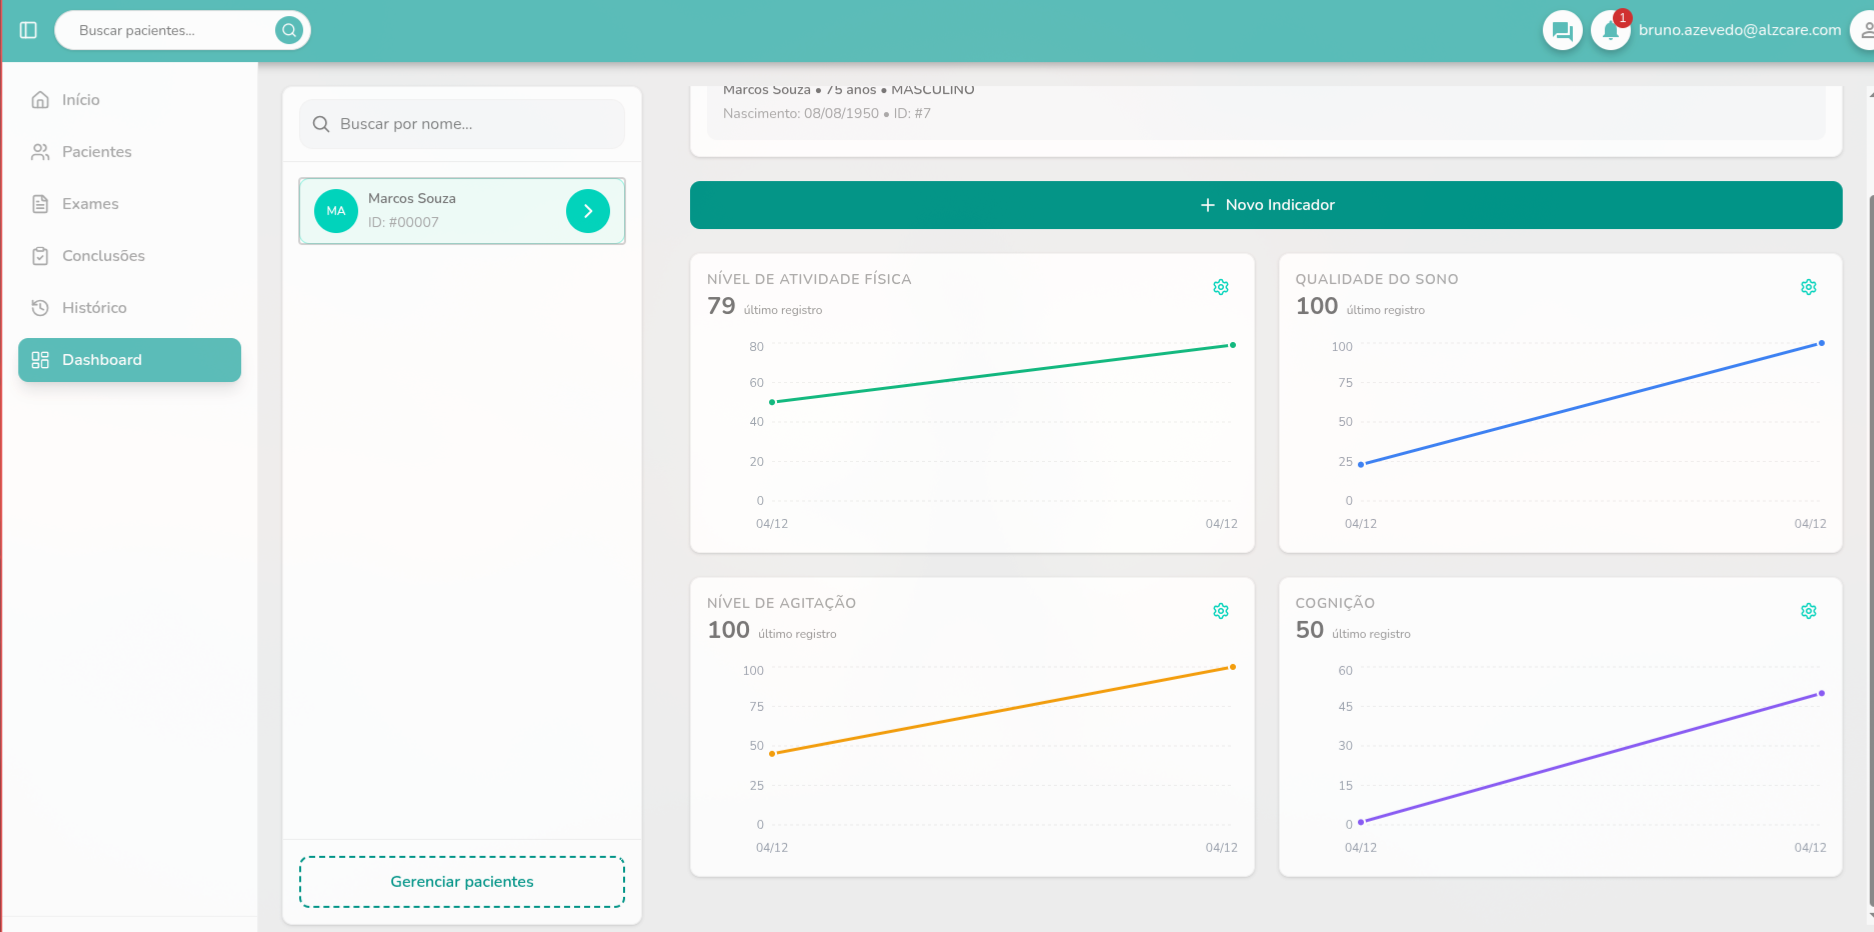
\includegraphics[height=5cm]{images/Prints/indicadores.png}}
    \label{fig:indicadorWeb}
    \vspace{2mm}
    {\footnotesize Fonte: Os autores (2025)}
\end{figure}

No coração da plataforma está o \emph{Prontuário Digital Integrado}. Ao abrir o perfil de um paciente, o médico encontra um dashboard consolidado com indicadores essenciais (dados cadastrais, contatos, alertas clínicos) e uma linha do tempo cronológica (\emph{timeline}) que unifica, de forma facilmente navegável:
\begin{itemize}
    \item consultas realizadas e agendadas, com status e possibilidade de reagendamento;
    \item histórico de exames solicitados e seus respectivos status de processamento;
    \item resultados de exames enviados pelos cuidadores (PDFs e imagens), com visualização inline e opção de download;
    \item anotações clínicas e observações diárias registradas por cuidadores ou pela própria equipe.
\end{itemize}

A interface permite registrar conclusões, prescrever condutas e solicitar novos exames diretamente no prontuário, reduzindo cliques e melhorando a produtividade. Recursos adicionais incluem histórico de ações (\textit{audit trail}), controle de versões nas notas clínicas e integração com mecanismo de notificações para alertar sobre novos documentos ou mensagens relevantes.

Outro aspecto relevante da interface Web é a otimização do fluxo de trabalho médico através da centralização de dados heterogêneos. Ao permitir a visualização simultânea de notas clínicas anteriores e novos resultados de exames na mesma janela de visualização, o sistema reduz a necessidade de alternância entre telas e documentos físicos, mitigando a carga cognitiva durante a consulta. Essa disposição estratégica das informações favorece a análise comparativa longitudinal, permitindo que o profissional identifique com maior agilidade padrões de estabilidade ou declínio cognitivo ao longo do tempo. Dessa forma, a plataforma não atua apenas como um repositório passivo, mas como uma ferramenta ativa de suporte à decisão, fundamentando ajustes medicamentosos ou novas intervenções terapêuticas com base em um histórico consolidado e acessível.

\subsubsection{Aplicativo Móvel (Paciente e Cuidador)}
O aplicativo móvel foi desenvolvido para máxima simplicidade, facilitando o engajamento do cuidador e a adesão do paciente ao acompanhamento. O aplicativo móvel foi projetado com ênfase na ergonomia cognitiva, visando reduzir barreiras tecnológicas e maximizar o engajamento tanto de cuidadores quanto de pacientes. A interface principal atua como um painel de controle intuitivo, onde a arquitetura da informação prioriza tarefas críticas e pendências imediatas. Através de um sistema de \textit{cards} visuais e notificações proativas, o sistema garante que solicitações de exames, mensagens da equipe médica e lembretes de medicação sejam visualizados prontamente, apoiando a adesão rigorosa ao tratamento. A fluidez e simplicidade do fluxo de uso são evidenciadas na funcionalidade de envio e anexo de documentos, que permite o encaminhamento rápido de exames diretamente pelo aplicativo, minimizando etapas e possíveis erros operacionais. A Figura~\ref{fig:examMobile} ilustra a interface destinada ao anexo de exames no aplicativo móvel, demonstrando a clareza visual e a objetividade do processo.

\begin{figure}[H]
    \centering
    \caption{Anexo de Exames do aplicativo móvel.}
    \makebox[\columnwidth][c]{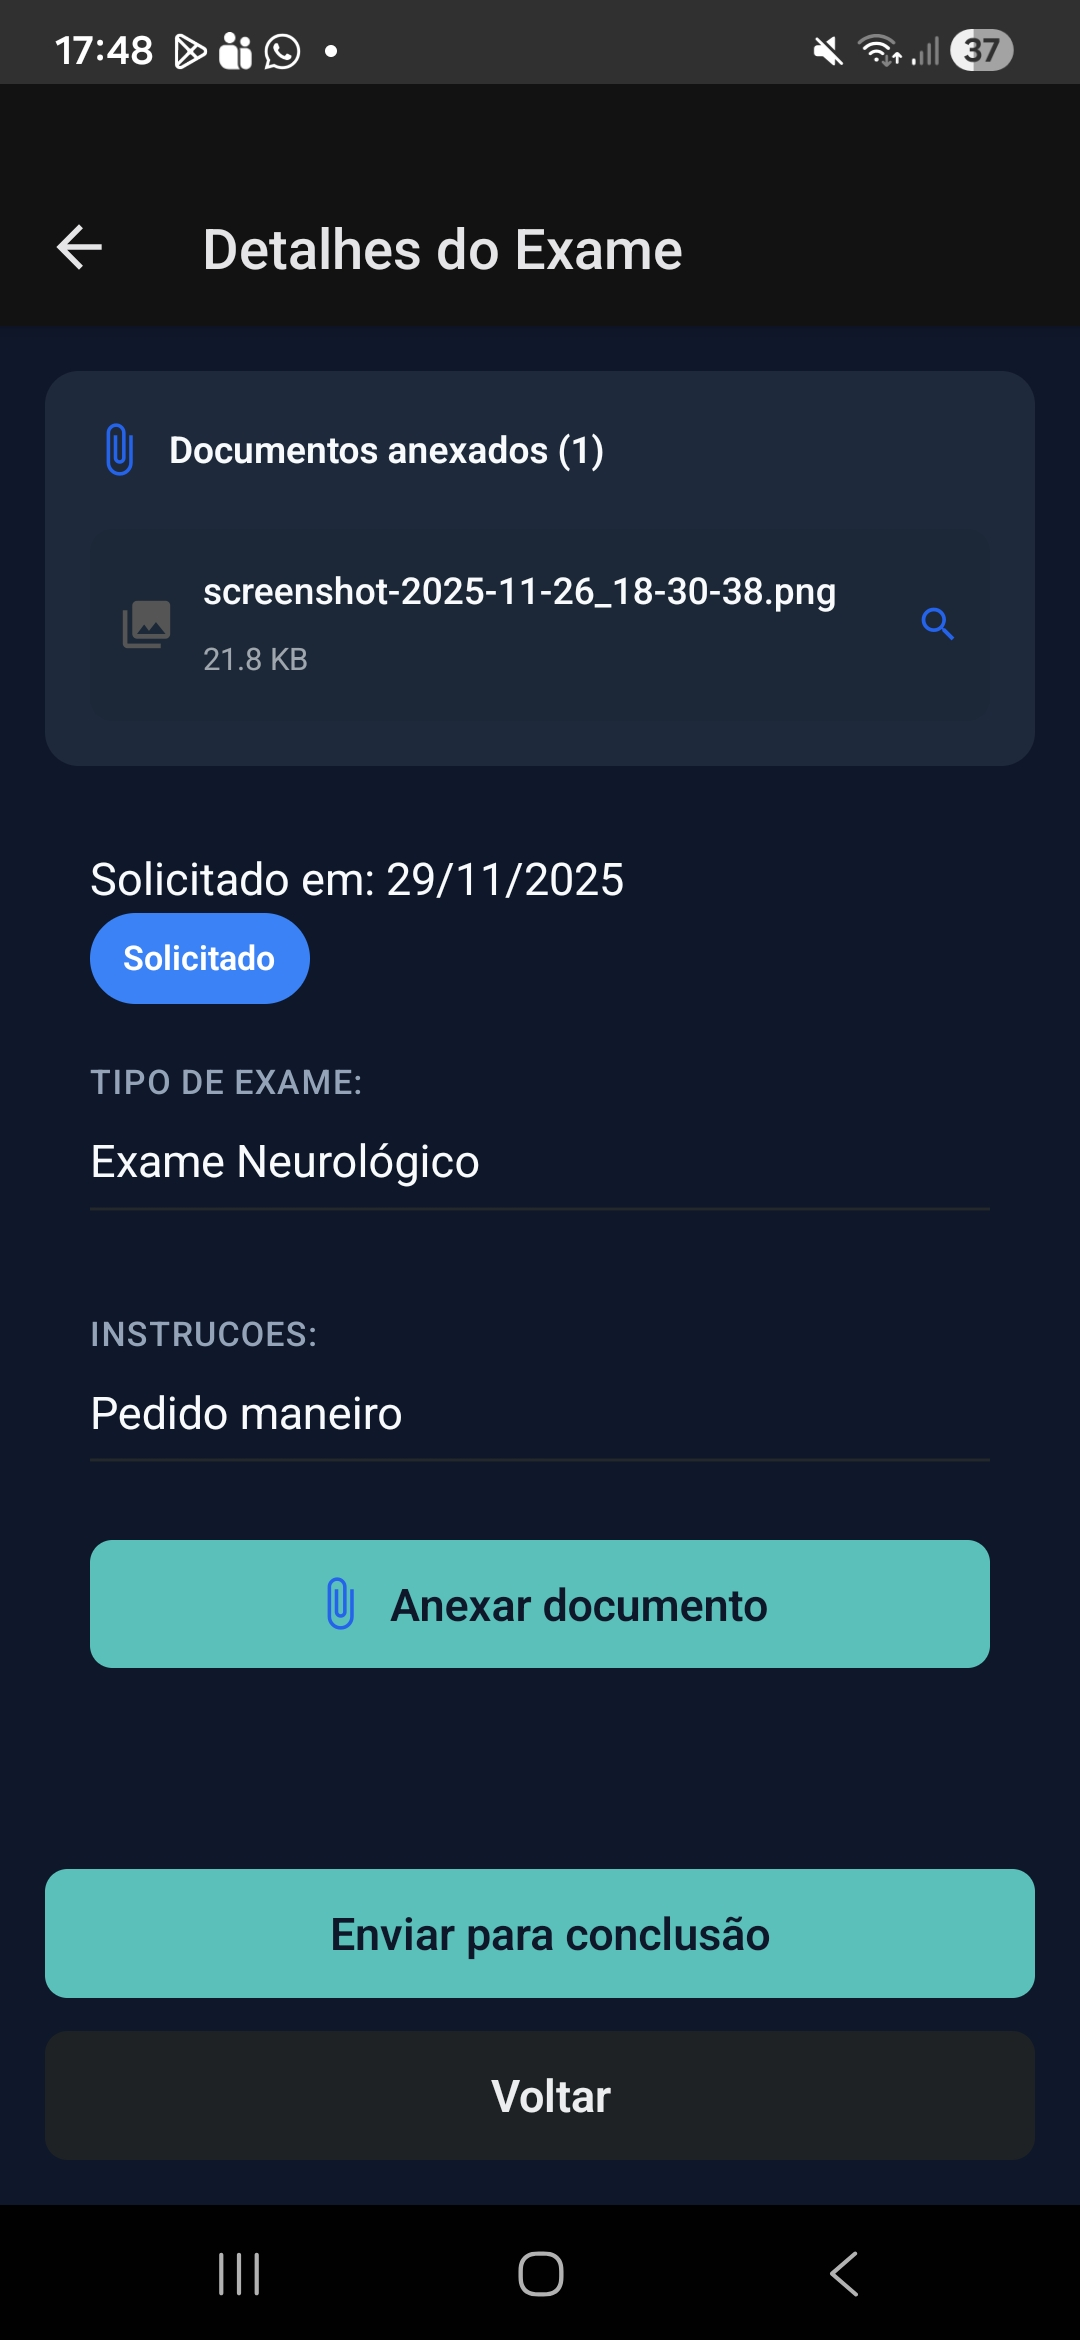
\includegraphics[height=10cm]{images/Prints/Screenshot_20251204_174832_front-end.jpg}}
    \label{fig:examMobile}
    \vspace{2mm}
    {\footnotesize Fonte: Os autores (2025)}
\end{figure}

Com o objetivo de garantir comunicação segura, ágil e rastreável entre a equipe de saúde e os cuidadores, o aplicativo móvel incorpora um módulo de chat protegido, desenvolvido com mecanismos de segurança que asseguram a confidencialidade das informações trocadas. Esse módulo permite a troca de mensagens em tempo quase real, o envio de orientações clínicas, esclarecimento de dúvidas e acompanhamento contínuo do paciente, além de disponibilizar indicadores visuais de mensagens não lidas, facilitando a identificação de pendências comunicacionais.O processo de envio de documentos foi projetado para ser simples e eficiente, reduzindo o esforço do cuidador e minimizando erros operacionais. O usuário pode capturar imagens diretamente pela câmera do dispositivo ou anexar arquivos já armazenados, associando-os de forma explícita à respectiva solicitação de exame. O sistema realiza a validação automática dos formatos permitidos (PDF ou imagem), executa o \textit{upload} de forma cifrada para a nuvem e disponibiliza o conteúdo de maneira imediata e integrada ao prontuário do paciente na plataforma Web, permitindo o acesso instantâneo pelo profissional de saúde.
Na Figura~\ref{fig:chatMobile}, é apresentada a interface do módulo de chat do aplicativo móvel, evidenciando sua organização visual, clareza na disposição das mensagens e foco na usabilidade, fatores essenciais para uma comunicação eficaz no contexto do acompanhamento clínico.

\begin{figure}[H]
    \centering
    \caption{Chat do aplicativo móvel.}
    \makebox[\columnwidth][c]{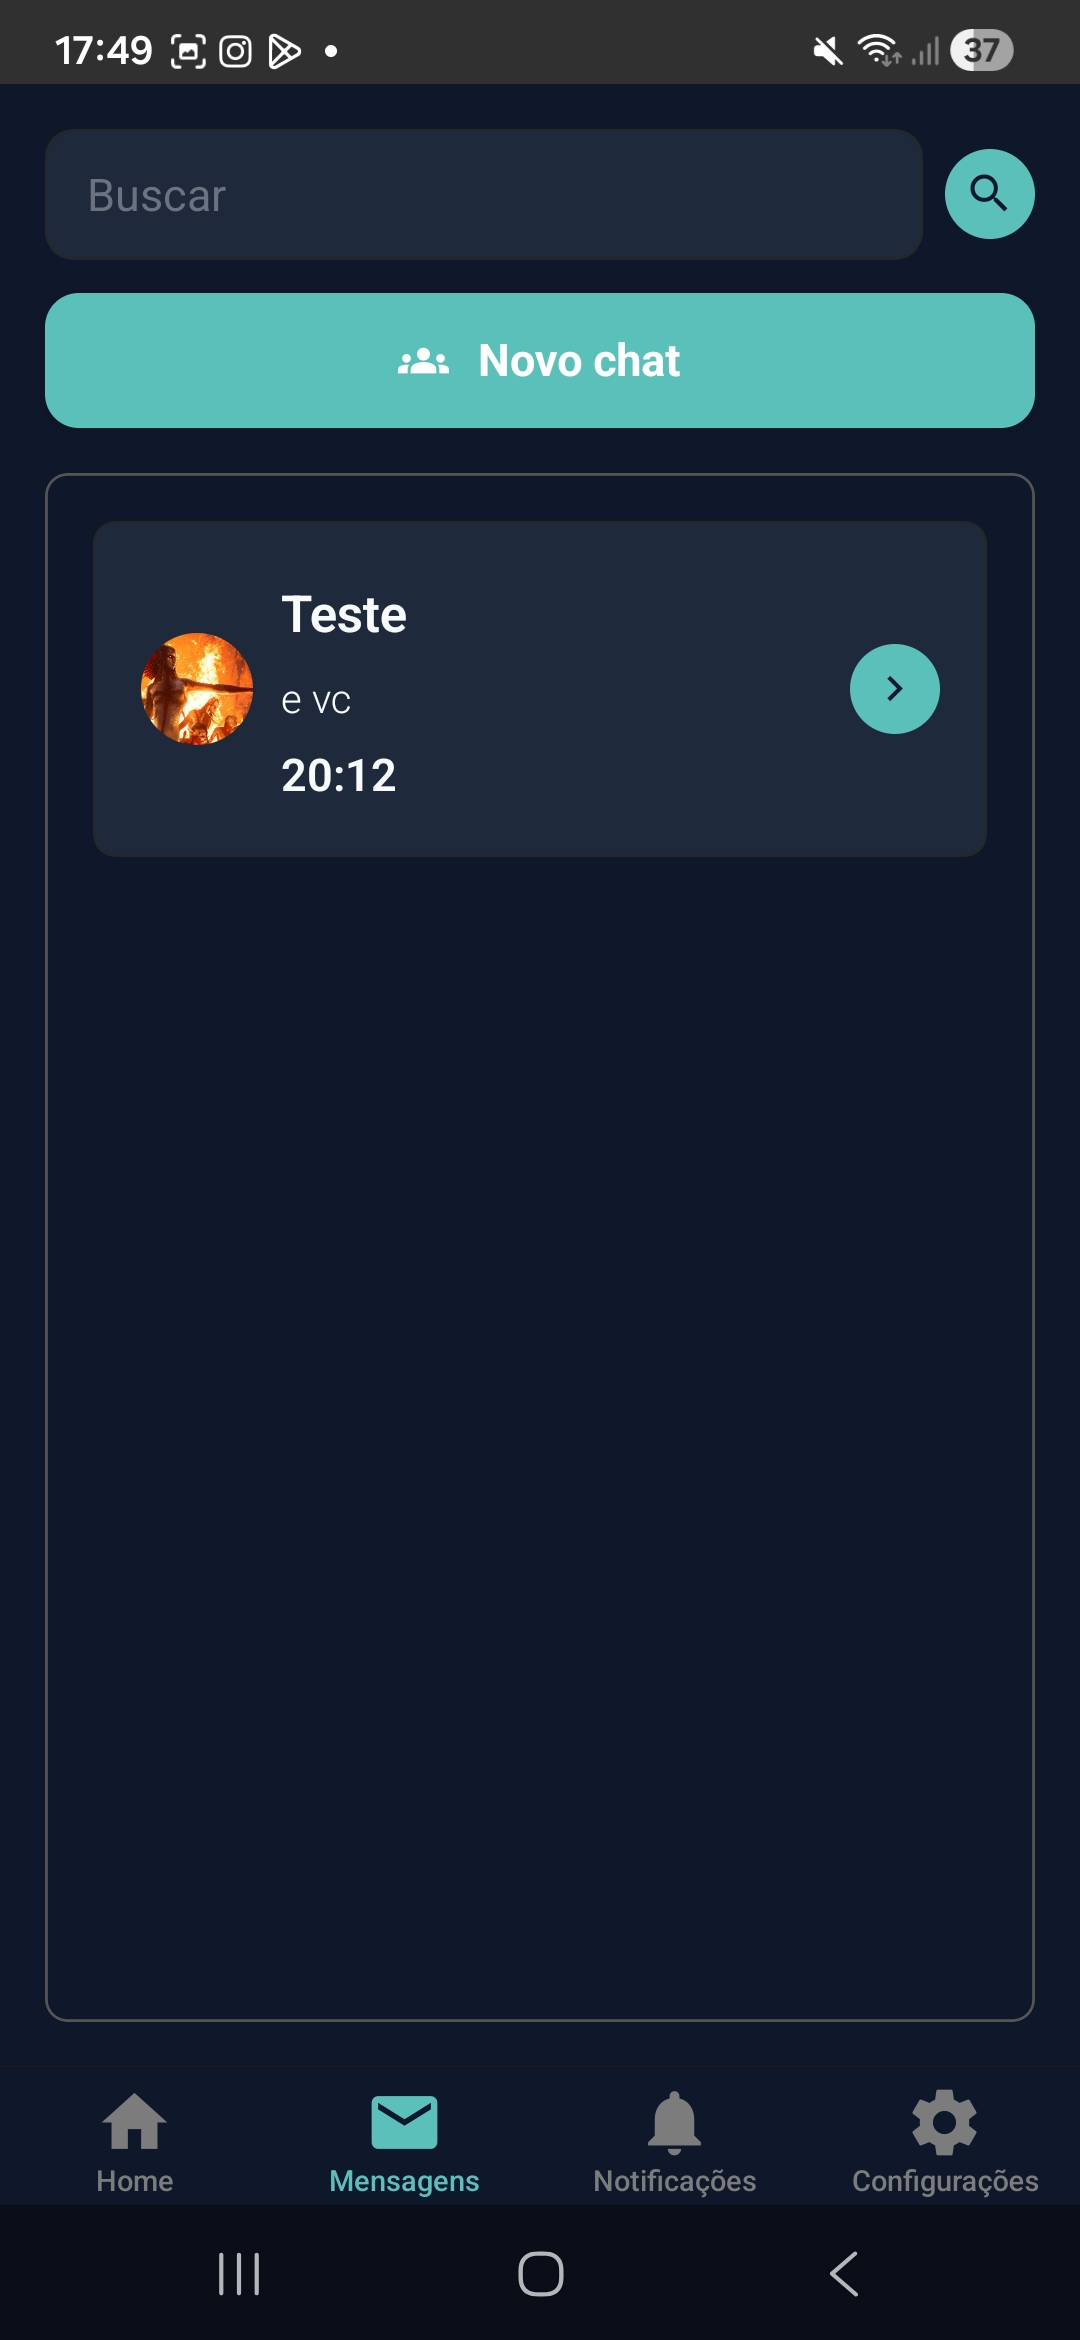
\includegraphics[height=10cm]{images/Prints/Screenshot_20251204_174904_front-end.jpg}}
    \label{fig:chatMobile}
    \vspace{2mm}
    {\footnotesize Fonte: Os autores (2025)}
\end{figure}

Além disso, o aplicativo prioriza acessibilidade (texto legível, botões de toque ampliados, fluxo reduzido de telas) e otimizações para conexões móveis, garantindo que \textit{uploads} e mensagens sejam retomados quando a rede for restabelecida. Notificações e alertas reforçam o acompanhamento contínuo e apoiam a coordenação do cuidado entre todos os envolvidos. A organização visual do aplicativo adota uma hierarquia clara de informações, onde os elementos mais urgentes, como pendências de exames e mensagens não lidas, são destacados no topo da interface para imediata visualização. A navegação entre os módulos principais é realizada através de uma barra inferior persistente, permitindo que o usuário alterne rapidamente entre o chat, as notificações e o perfil do paciente sem perder o contexto de navegação. Para assegurar a fluidez no uso diário, o fluxo de cadastro de informações foi segmentado em etapas curtas e objetivas, evitando a sobrecarga cognitiva do cuidador durante o preenchimento de dados. O design responsivo implementado garante ainda que a disposição dos elementos se adapte automaticamente a diferentes tamanhos de tela e densidades de pixels, mantendo a integridade do layout em diversos dispositivos móveis.

A integração entre as plataformas Web e móvel promove uma orquestração eficiente do fluxo de informações clínicas, contribuindo diretamente para a redução de atrasos no diagnóstico por meio do envio rápido e estruturado de resultados, além de favorecer uma comunicação mais fluida e contínua entre profissionais de saúde, cuidadores e pacientes. Essa integração também assegura maior rastreabilidade das ações realizadas, permitindo o acompanhamento histórico de interações, solicitações e respostas ao longo do processo clínico.O conjunto de funcionalidades foi concebido para aprimorar a tomada de decisão clínica e a experiência do usuário final, com ênfase em princípios de segurança da informação, clareza na apresentação dos dados e agilidade operacional. As informações são sincronizadas entre os ambientes de forma consistente, garantindo que profissionais e cuidadores tenham acesso a dados atualizados e confiáveis.

Conforme ilustrado na Figura~\ref{fig:notifyMobile}, o aplicativo móvel disponibiliza um módulo de notificações detalhadas, no qual cada alerta é contextualizado e direciona o usuário diretamente para a entidade ou funcionalidade relacionada, como exames, mensagens ou solicitações específicas. Esse mecanismo reduz o tempo de navegação, evita perdas de informação relevante e reforça a eficiência do acompanhamento clínico.

\begin{figure}[H]
    \centering
    \caption{Notificações no aplicativo móvel.}
    \makebox[\columnwidth][c]{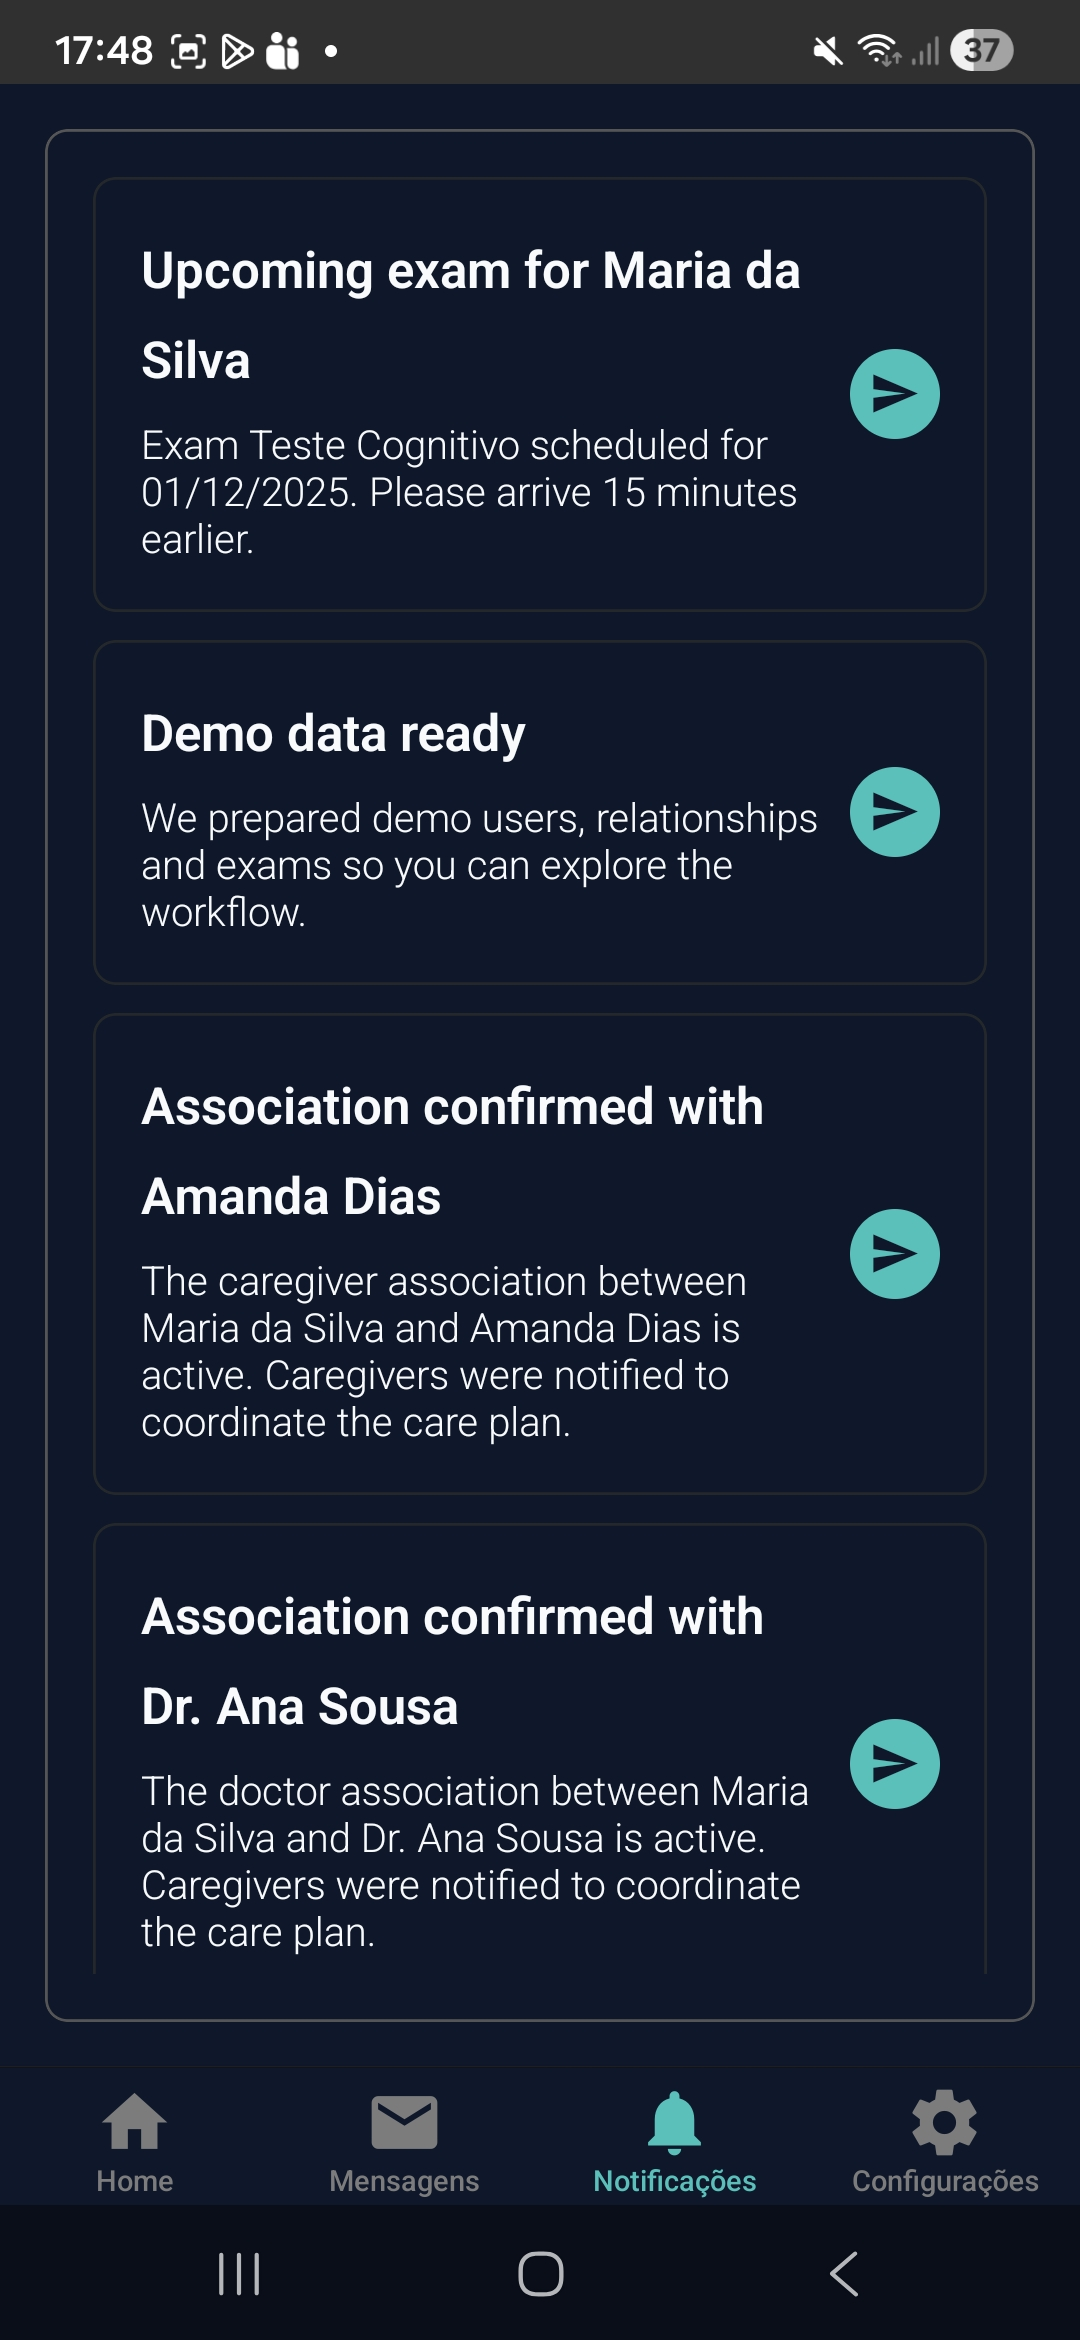
\includegraphics[height=10cm]{images/Prints/Screenshot_20251204_174844_front-end.jpg}}
    \label{fig:notifyMobile}
    \vspace{2mm}
    {\footnotesize Fonte: Os autores (2025)}
\end{figure}









%=============================================================================%
%============================== Secao 5 ======================================%
%=============================================================================%


\section{CONSIDERAÇÕES FINAIS}
O presente trabalho dedicou-se ao desenvolvimento de um sistema de acompanhamento para pessoas com a Doença de Alzheimer, uma condição neurodegenerativa que impõe desafios significativos não apenas aos pacientes, mas também a seus familiares, cuidadores e ao sistema de saúde como um todo. A crescente prevalência do Alzheimer, com estimativas de que o número de casos ultrapasse 150 milhões até 2050, somada à complexidade de seu manejo, evidencia a necessidade crítica de soluções inovadoras que possam aprimorar o cuidado e o monitoramento contínuo desses pacientes. 

O problema central abordado foi a dificuldade em acompanhar a progressão lenta e variável da doença, o que impede ajustes oportunos nas intervenções médicas e a antecipação de eventos adversos, sobrecarregando os cuidadores e comprometendo a segurança do paciente. Diante disso, o objetivo geral do projeto foi desenvolver uma solução tecnológica integrada, composta por uma plataforma web para médicos e um aplicativo móvel para pacientes e cuidadores, visando otimizar o monitoramento, a comunicação e a gestão do tratamento. 

Para alcançar este objetivo, o projeto foi estruturado para cumprir metas específicas, como o desenvolvimento de um dashboard com o histórico completo do paciente para o médico, a implementação de um chat para comunicação direta, a funcionalidade de anexo de exames e históricos pelo aplicativo móvel, e um sistema de notificações para manter todos os envolvidos atualizados. A plataforma foi concebida para centralizar as informações e facilitar o acompanhamento detalhado, fatores cruciais para a eficácia das intervenções terapêuticas. 

A metodologia de desenvolvimento adotada baseou-se em práticas ágeis, como o Scrum e o Kanban, que permitiram um gerenciamento de projeto flexível e iterativo, com entregas de valor contínuas ao longo de Sprints. A modelagem do sistema foi realizada com o auxílio da linguagem UML, por meio de diagramas de Casos de Uso, Sequência, Classes e Entidade-Relacionamento, que garantiram uma base sólida e bem-documentada para a construção do software. 

A arquitetura da solução foi projetada como um sistema nativo em nuvem, utilizando a plataforma Microsoft Azure para garantir escalabilidade, segurança e resiliência. A tecnologia empregada reflete as práticas modernas de desenvolvimento de software, com o uso de React para a interface web, React Native para o aplicativo móvel multiplataforma e uma API RESTful robusta desenvolvida em Java com o framework Spring Boot. O armazenamento de dados foi dividido entre o PostgreSQL, para dados estruturados, e o Firebase Storage, para arquivos como exames e documentos. 

Conclui-se que o sistema proposto atende aos objetivos estabelecidos, oferecendo uma ferramenta valiosa e alinhada à crescente transformação digital no setor da saúde. A solução centraliza informações críticas, agiliza a comunicação e fornece aos médicos dados organizados para uma tomada de decisão mais eficaz, enquanto empodera pacientes e cuidadores com acesso facilitado às informações e ao suporte profissional. 

Entretanto, é importante ressaltar as limitações do escopo atual da solução. O sistema, neste estágio, não incorpora técnicas de Inteligência Artificial, dependendo inteiramente da entrada manual para a interpretação dos dados. Consequentemente, o módulo de exames atua como um repositório digital de anexos, sem realizar a extração automática de dados estruturados ou a leitura inteligente de laudos a partir dos arquivos enviados. Outra restrição refere-se ao perfil do paciente dentro da aplicação, atualmente, sua função opera primordialmente como um proxy (intermediário) de conexão entre o médico e o cuidador, possuindo baixa interatividade direta e poucas funcionalidades ativas no fluxo de uso.

Como trabalhos futuros, vislumbra-se a integração de algoritmos de machine learning para a predição de eventos críticos, como agitação e desorientação, com base nos históricos contextuais coletados, uma possibilidade já explorada na fundamentação teórica. Adicionalmente, a incorporação de dados provenientes de dispositivos vestíveis (wearables) poderia automatizar a coleta de informações sobre a atividade física e a qualidade do sono do paciente, enriquecendo ainda mais a análise médica e tornando o monitoramento mais proativo e menos invasivo. 

%%%%%%%%%%%%%%%%%%%%%%%%%%%%%%%%%%%%%%%%%%%%%%%%%%%%%%%%%%%%
% REFERÊNCIAS

\def\refname{Referências}

\bibliographystyle{abntex2-num}
\bibliography{referencias}



\end{document}
